\documentclass{beamer}
\usetheme{JuanLesPins}
%\usecolortheme{beaver}

\usepackage{fontspec}
\usepackage[spanish]{babel}

\title[Uso redes neuronales]{Uso de redes neuronales para la clasificación de células}
\subtitle{Trabajo innovación}

\author[Marc, Joan, Iñigo]{
	Marc Asenjo \and
	Joan Marcè \and
	Iñigo Moreno
	}
\institute[UPC]{Universitat Politècnica de Catalunya}
\date{2016}

\AtBeginSection[]
{
	\begin{frame}
		\frametitle{Contenido}
		\tableofcontents[currentsection,currentsubsection]
	\end{frame}
}

\AtBeginSubsection[]
{
	\begin{frame}
		\frametitle{Contenido}
		\tableofcontents[currentsection,currentsubsection]
	\end{frame}
}

\begin{document}

\frame{\titlepage}

\section{Introducción}

\section{Sistemas de clasificación celular}

\section{Ejemplos actuales}

\begin{frame}
	\begin{figure}
		\centering
		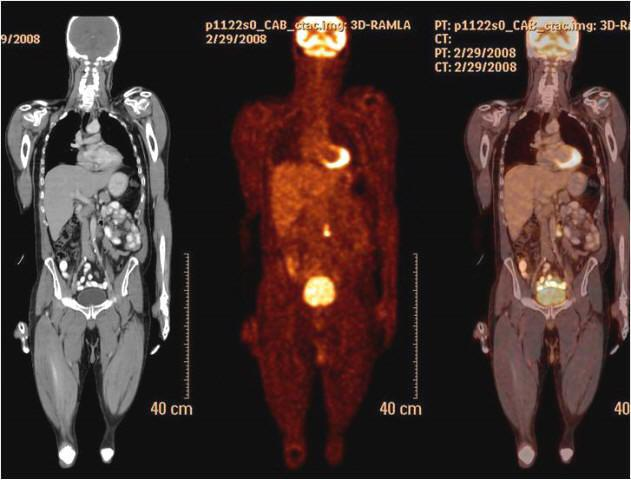
\includegraphics[width=.9\textheight]{intro_1}
	\end{figure}
\end{frame}

\section{Introducción al sistema de clasificación}

\subsection{Adquisición de datos}

\begin{frame}
	\begin{figure}
		\centering
		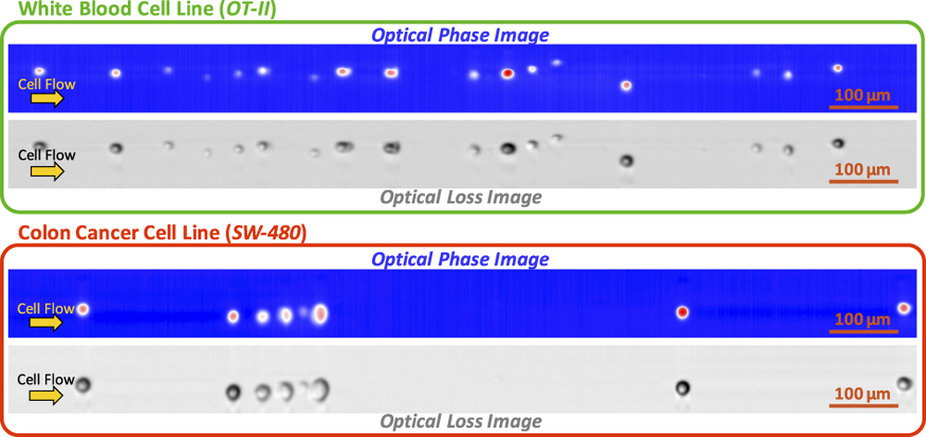
\includegraphics[width=\linewidth]{Phase}
	\end{figure}
\end{frame}

\subsection{Datos calculados}

\begin{frame}
	\begin{figure}
		\centering
		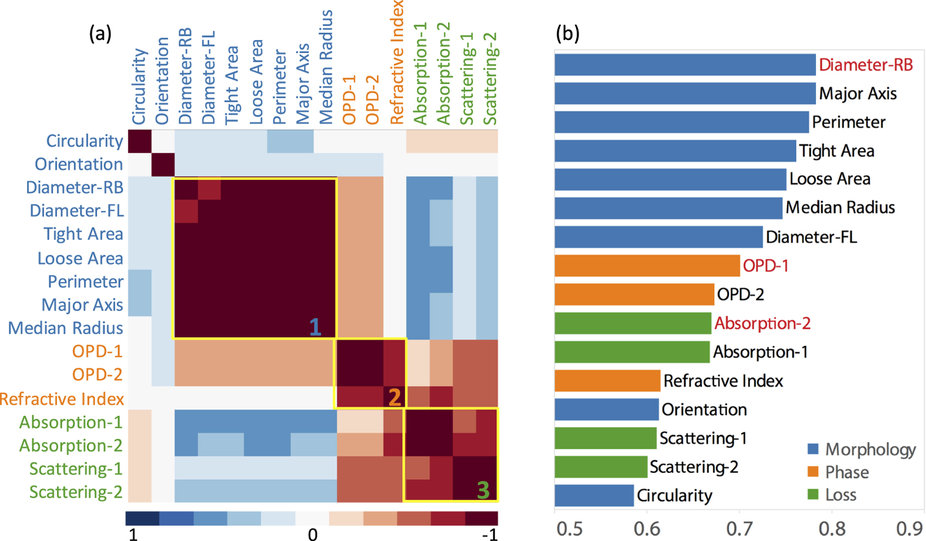
\includegraphics[width=\linewidth]{features}
	\end{figure}
\end{frame}
	
\section{Uso de tecnologías de inteligencia artificial}
	
\begin{frame}
	\begin{figure}
		\centering
		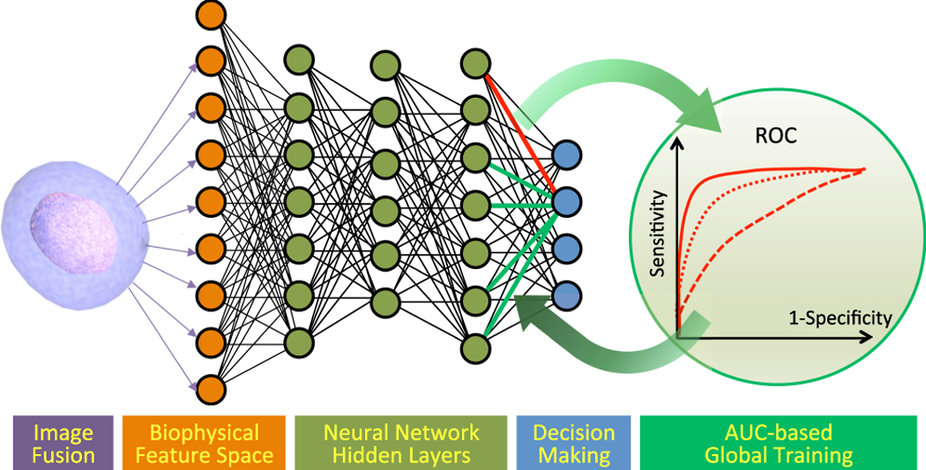
\includegraphics[width=\linewidth]{neural}
	\end{figure}
\end{frame}

\section{Impacto del descubrimiento}

\subsection{Impacto en el cáncer}

\begin{frame}
	\begin{figure}
		\centering
		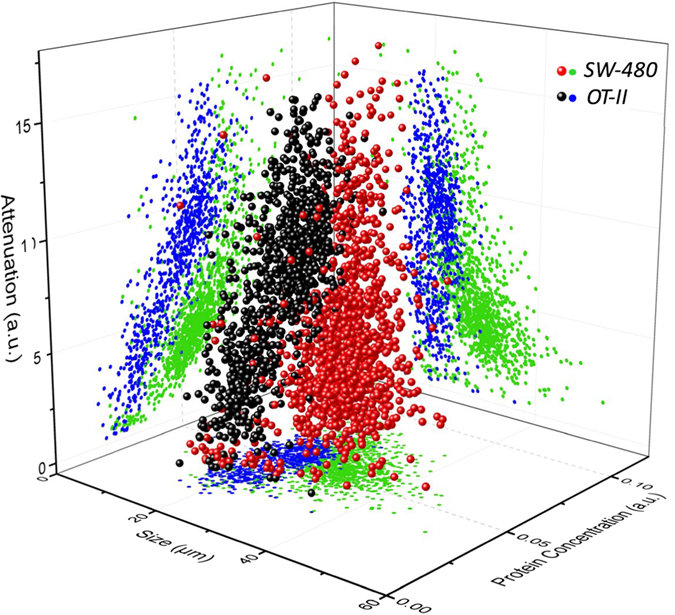
\includegraphics[height=.9\textheight]{impacto_1}
	\end{figure}
\end{frame}

\subsection{Impacto en el biodiésel}

\begin{frame}
	\begin{figure}
		\centering
		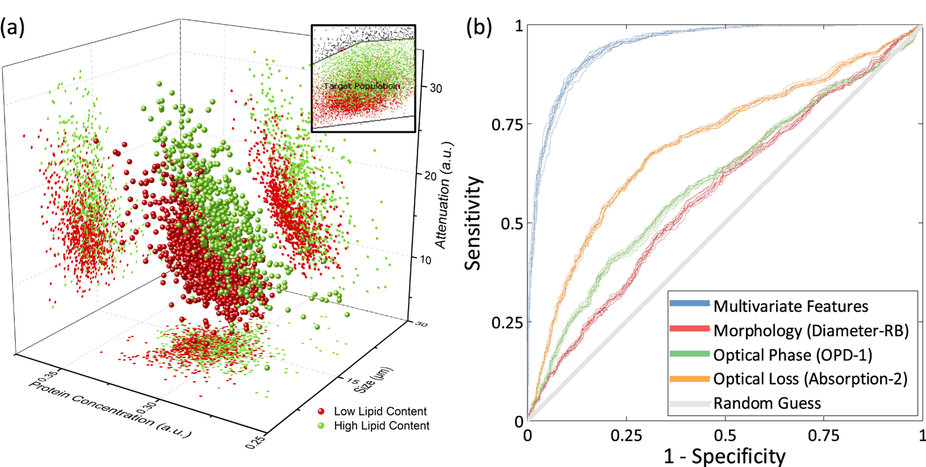
\includegraphics[width=\linewidth]{impacto_2}
	\end{figure}
\end{frame}
	
\end{document}